% Feature-first revision v9, 16 October 2026.
% Preserves v7 Figure 1; uses six left panels and one square peer-slope matrix spanning both rows.
% Source of record: accentuation_rmt_main_compact_draft.tex -> main_body_compact.tex.
% COSYNE rules verified at https://www.cosyne.org/abstracts-submission.
% 12 pt body, A4, 0.5 in margins; 10 pt captions/references; anonymous.
% Figure 1: notes/build_cosyne2027_dense_figures.py
% Figure 2: notes/build_cosyne2027_figure2_square.py
\documentclass[12pt,a4paper]{article}
\usepackage[margin=0.5in]{geometry}
\usepackage[T1]{fontenc}
\usepackage{times,amsmath,amssymb,graphicx,caption}
\usepackage[hidelinks]{hyperref}
\hypersetup{pdftitle={Why accurate neural predictions do not guarantee effective neural control},pdfauthor={},pdfsubject={COSYNE 2027: geometry-first theory with a square peer-slope matrix},pdfkeywords={}}
\pagestyle{empty}
\setlength{\parindent}{0pt}
\linespread{0.93}
\setlength{\parskip}{1.5pt}
\AtBeginDocument{%
  \setlength{\abovedisplayskip}{2pt}%
  \setlength{\belowdisplayskip}{2pt}%
  \setlength{\abovedisplayshortskip}{2pt}%
  \setlength{\belowdisplayshortskip}{2pt}%
}
\setlength{\emergencystretch}{1.5em}
\captionsetup{font=footnotesize,labelfont=bf,labelsep=period,skip=3pt,hypcap=false}
\newcommand{\head}[1]{\par\noindent\textbf{#1}\enspace\ignorespaces}
\newcommand{\bh}{\hat\beta}
\newcommand{\bt}{\beta^\star}
\newcommand{\mb}{\bar\beta}
\begin{document}
{\large\bfseries Why accurate neural predictions do not guarantee effective neural control\par}

\textbf{Summary.}
Encoding models of visual cortex can predict natural-image responses yet fail to generate images that control them. Motivated by a closed-loop comparison of ten models at 25 sites in five macaques, we develop a regression theory of this dissociation. Prediction samples the training distribution; control follows the model's own optimized directions, where low natural-image variance can conceal estimation errors. Random matrix theory shows how finite data and noisy responses inflate model-predicted gain without increasing neural gain, and why prediction-selected regularization need not prevent this failure. Fixed feature maps can preserve prediction while changing control arbitrarily; a gradient-geometry factor isolates this additional sensitivity. Its nonlinear analogue correlates with biological control when held-out error is largely uninformative. The theory also explains how poor generators recognize effective stimuli from other models. The resulting decomposition suggests how data collection, noise reduction, and feature-gradient geometry can guide more reliable control.

\head{The experimental puzzle.}
Prince, Wang, et al.~[1] recorded naturalistic-image responses at 25 sites in five macaques, spanning V3/V4, inferotemporal cortex (IT) and superior temporal sulcus (STS). For each of ten fixed deep-network backbones $\phi_m$, cross-validated ridge regression fitted a linear readout, $f_m(x)=\hat w_m^\top\phi_m(x)$. Feature accentuation~[2] then modified each seed image using regularized gradient ascent or descent on $f_m$ to reach graded response targets within and beyond the neuron's natural-image range (Fig.~\ref{fig:experiment}A). Presenting these images to the same sites tested whether measured responses matched the model's targets. Despite similar natural-image predictivity, trained models differed sharply in control (Fig.~\ref{fig:experiment}E,F); an accurate predictor could barely modulate its target site (Fig.~\ref{fig:experiment}B--D). Unsuccessful controllers could still predict responses to another model's effective stimuli.

\par\noindent\begin{minipage}{\linewidth}\centering
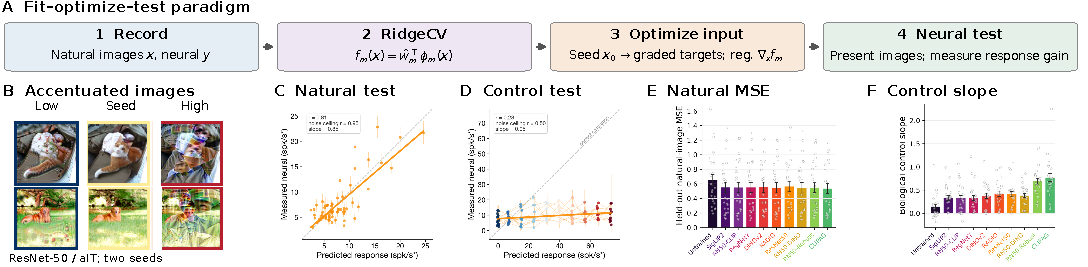
\includegraphics[width=\linewidth]{figures/cosyne2027_v7_experiment_dense.pdf}
\captionof{figure}{\textbf{From encoding to control.} \textbf{A}~RidgeCV on fixed features, regularized input-gradient optimization, and neural testing. \textbf{B--D}~One ResNet-50/aIT site from~[1]: two accentuation sweeps; natural test responses ($r=0.81$, slope $0.85$); control responses ($r=0.28$, slope $0.05$). \textbf{E,F}~Natural-image MSE and control slope across ten models: sites (dots), mean and $\pm1$~SE (bars); 25 sites.}
\label{fig:experiment}
\end{minipage}\par

\head{From experiment to a solvable model.}
We preserve the backbone--readout structure but replace $\phi(x)$ by fixed linear features $Fx$. Natural inputs $x\sim\mathcal N(0,\Sigma)$ drive a noisy linear neuron, $y=x^\top\bt+\sigma\epsilon$, with independent unit-variance noise $\epsilon$. Ridge regression on $n$ examples fits $f(x)=\hat w^\top Fx=x^\top\bh$, with pixel gradient $\bh=F^\top\hat w$ (Fig.~\ref{fig:evidence}A). We retain ridge fitting but idealize regularized synthesis as the straight path $x=x_0+\alpha\bh$. From a centered seed $x_0=0$, mean neural and predicted response changes are $\alpha N$ and $\alpha D$:
\begin{equation}
\mathrm{slope}_{\rm control}=\frac ND=
\frac{\bh^\top\bt}{\|\bh\|^2}\,
\begin{subarray}{l}
\text{actual neural gain}\\[8pt]
\text{model-predicted gain}
\end{subarray},
\qquad R^2_{\rm control}=1-\left(\frac DN-1\right)^2.
\label{eq:geometry}
\end{equation}
Alignment $N$ is the actual neural gain; squared norm $D$ is the model's claimed gain. For $N>0$, $D<N$ means underprediction (slope $>1$), $D=N$ means perfect calibration, and $D>N$ means overprediction (slope $<1$), which could lead to negative $R^2$ (when $D>2N$). Natural-image prediction instead measures $E_{\rm gen}=(\bh-\bt)^\top\Sigma(\bh-\bt)$, downweighting low-variance directions. Errors along these directions can therefore inflate the model's claimed gain $D$ with little predictive cost or corresponding neural gain $N$.

\head{Why cross-validation does not remove the problem.}
The failure already occurs for $F=I$, with no backbone geometry. Random matrix theory~[3] gives leading approximations as dimension and sample size grow proportionally. The mean weight is the teacher shrunk along each covariance eigenvector:
\begin{equation}
\mb:=\Sigma(\Sigma+\kappa I)^{-1}\bt
=\sum_k\frac{s_k}{s_k+\kappa}\,b_k u_k,
\qquad \Sigma u_k=s_k u_k,\quad b_k=u_k^\top\bt.
\label{eq:mean-shrinkage}
\end{equation}
Here $\kappa$ is the effective ridge penalty accounting for finite sampling; each shrinkage factor $s_k/(s_k+\kappa)\in[0,1]$.\par
Finite-data fluctuations inflate squared norm $D$ by $V$, without changing leading alignment $N$:
\begin{equation}
\mathrm{slope}_{\rm control}\simeq
\frac{\mb^\top\bt}{\|\mb\|^2+V},
\qquad
V=\frac{E_{\rm gen}+\sigma^2}{n}
\sum_k\frac{s_k}{(s_k+\kappa)^2},
\label{eq:inflation}
\end{equation}\par
For the mean alone, $\|\mb\|^2\le\mb^\top\bt$: the student underpredicts. Inflation increases the model-predicted gain $D$ without increasing the neural gain $N$. It first compensates for shrinkage, giving $D=N$, then causes overprediction once $D>N$.\par
Prediction-optimal and control-calibrated penalties satisfy different spectral conditions for anisotropic inputs and a structured teacher. Natural-image simulations confirm that cross-validation preserves good prediction while control deteriorates (Fig.~\ref{fig:evidence}B,C).\par

\head{Why equally predictive feature maps control differently.}
For general $F$, prediction depends on the feature covariance $F\Sigma F^\top$ and its relationship to the teacher; control also depends on how features map back into pixels $FF^\top$. We construct transformations preserving the joint feature--response distribution, hence the predicted generalization curve and its optimal penalty stay invariant, while control changes (Fig.~\ref{fig:evidence}D). Increasing input anisotropy can make this dissociation arbitrarily severe.

The feature-gradient geometry enters the norm inflation, 
\begin{equation}
V_F=\frac{E_{\rm gen}+\sigma^2}{n}\,T_F(\kappa),
\qquad
T_F(\kappa)=\sum_{k:s_k>0}
\left(\frac{s_k}{s_k+\kappa}\right)^2
\frac{\|g_k\|^2}{g_k^\top\Sigma g_k},
\label{eq:features}
\end{equation}
where $(s_k,v_k)$ now denote feature-covariance eigenpairs and $g_k=F^\top v_k$ is a feature direction's pixel gradient. The sum weights features that survive regularization and compares their gradient energy with natural-image variation along that gradient. Thus, control is fragile when well-estimated features send their gradients into weakly constrained pixel directions, making $T_F$ large without changing prediction error.

\head{From linear theory to biological control.}
For nonlinear features $\phi$, the corresponding diagnostic uses the feature Jacobian $J_\phi$ at seed images: $T_\phi=\sum_k s_k/(s_k+\kappa)^2\|J_\phi(x)^\top v_k\|^2$. %we retain the spectral weights $s_k/(s_k+\kappa)^2$ and measure squared pixel-gradient norms $\|J_\phi(x)^\top v_k\|^2$. 
% their weighted sum, averaged over ten seeds, gives $T_\phi$, 
This diagnostic can be computed from the fitted model before a control experiment. Across nine trained models at 25 sites (225 site--model pairs), $\log_{10}T_\phi$ correlates with site-centered control slope at $r=-0.61$, compared with $r=0.02$ for log held-out mean squared error (Fig.~\ref{fig:evidence}F). This supports our heuristic nonlinear extension as a prognostic predictor of control success. %This association weakens substantially without the two adversarially trained models. It supports the diagnostic descriptively; the nonlinear extension is not a proved control-error formula.

\par\noindent\begin{minipage}{\linewidth}\centering
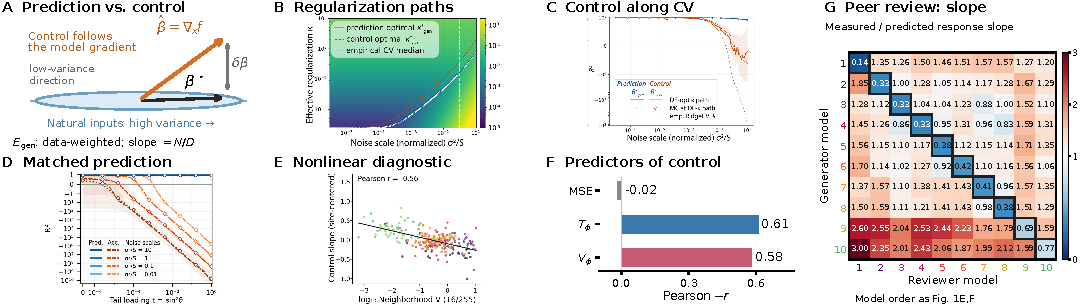
\includegraphics[width=\linewidth]{figures/cosyne2027_v9_square_matrix.pdf}
\captionof{figure}{\textbf{Prediction geometry and peer evaluation.} \textbf{A}~Schematic: low-variance input directions hide weight errors exposed by model gradients. \textbf{B,C}~Natural-image ridge ($d=10^4$, $n=10^3$): prediction-error landscape and prediction/control $R^2$ along the prediction-optimal path; dotted: empirical RidgeCV. \textbf{D}~Feature rotations preserve prediction while changing control. \textbf{E}~Neighborhood $V_\phi$ versus site-centered slope (ten models, 25 sites; $r=-0.56$). \textbf{F}~Log-predictor correlations for nine trained models. \textbf{G}~Peer slope averaged over 25 sites: generator rows, reviewer columns; boxed diagonal: self; model order as Fig.~\ref{fig:experiment}E,F. Correlations are descriptive.}
\label{fig:evidence}
\end{minipage}\par

\head{Recognition without generation.}
For independent pixel-space ridge fits at the same penalty, fluctuations cancel in the peer weight cross-product, removing the leading self-norm inflation: $D_{\rm peer}\simeq\|\mb\|^2\le\mb^\top\bt\simeq N_{\rm peer}$. Thus peer evaluation underpredicts (leading slope $\ge1$, $R^2\ge0$), while self-evaluation can overpredict with negative $R^2$. Reanalysis of neural data from~[1] supports this contrast: 80 of 90 peer slopes exceed one; median peer slope and $R^2$ are $1.35$ and $0.04$, versus $0.38$ and $-4.17$ for self-evaluation (Fig.~\ref{fig:evidence}G).

\head{Toward more reliable neural control.}
The factorization $V_F=(E_{\rm gen}+\sigma^2)T_F/n$ turns the failure mechanism into a design guide. It motivates better predictive fits, more training images, and trial averaging or denoising to reduce response noise. At a fixed effective penalty, $T_F$ adds a distinct criterion: among comparably predictive backbones, favor or regularize feature maps whose gradients place less energy in low-variance image directions. The nonlinear diagnostic makes this criterion testable before synthesis. Reducing inflation addresses overprediction; calibration still requires balancing it against shrinkage. The design target is calibrated gain: optimized images should change neural responses by as much as the model predicts.

\vspace{2pt}
{\fontsize{10}{11}\selectfont
\textbf{References.}
[1] Prince, Wang, et al. (2026). Parametric neural control differentiates top neural network models of primate visual cortex. \emph{bioRxiv}, doi:10.64898/2026.08.16.745063.
[2] Hamblin et al. (2024). Feature accentuation: Revealing `what' features respond to in natural images. arXiv:2402.10039.
[3] Dobriban \& Wager (2018). High-dimensional asymptotics of prediction: Ridge regression and classification. \emph{Annals of Statistics} 46:247--279.
\par}
\end{document}
